\newcounter{exno}
\def\exercise{\bigskip\noindent\addtocounter{exno}{1}Exercício~\arabic{exno}.~}


typedef struct HeapTupleFields
{
  TransactionId t_xmin; /* inserting xact ID */
  TransactionId t_xmax; /* deleting or locking xact ID */
  union
  {
    CommandId t_cid; /* inserting or deleting command ID, or both */
    TransactionId t_xvac; /* VACUUM FULL xact ID */
  } t_field3;
} HeapTupleFields;
typedef struct HeapTupleHeaderData
{
  union
  {
    HeapTupleFields t_heap;
    DatumTupleFields t_datum;
  } t_choice;
  ItemPointerData t_ctid; /* current TID of this or newer tuple */
  /* Fields below here must match MinimalTupleData! */
  uint16 t_infomask2; /* number of attributes + various flags */
  uint16 t_infomask; /* various flag bits, see below */
  uint8 t_hoff; /* sizeof header incl. bitmap, padding */
  bits8 t_bits[1]; /* bitmap of NULLs −− VARIABLE LENGTH */
  /* ^ − 23 bytes − ^ */
  /* MORE DATA FOLLOWS AT END OF STRUCT */
  bits8 t_bits[1]; /* bitmap of NULLs −− VARIABLE LENGTH */
} HeapTupleHeaderData; /* 24 bytes */


typedef struct PageHeaderData
{
  /* XXX LSN is member of *any* block, not only page-organized ones */
  PageXLogRecPtr pd_lsn;  /* 8 bytes */        /* LSN: next byte after last byte of xlog
  * record for last change to this page */
  uint16          pd_checksum; /* 2 bytes */   /* checksum */
  uint16          pd_flags;   /* 2 bytes */            /* flag bits, see below */
  LocationIndex pd_lower;   /* 2 bytes */      /* offset to start of free space */
  LocationIndex pd_upper;    /* 2 bytes */     /* offset to end of free space */
  LocationIndex pd_special;   /* 2 bytes */    /* offset to start of special space */
  uint16          pd_pagesize_version; /* 2 bytes */
  TransactionId pd_prune_xid; /* 4 bytes */ /* oldest prunable XID, or zero if none */
  ItemIdData      pd_linp[FLEXIBLE_ARRAY_MEMBER]; /* 4 bytes */ /* line pointer array */
} PageHeaderData; /* 26 bytes */


\section*{Estruturas de armazenamento de indexação}

Utilize os seguintes dados para responder às questões: no PostgreSQL,
a tupla é composta por um cabeçalho de 24 bytes e seus campos.  As
tuplas são armazenadas em páginas de 8.192 bytes, onde cada página
possui um cabeçalho de 26 bytes e um vetor de ponteiros para cada
tupla com 4 bytes para cada elemento. Supondo que o banco de dados
está armazenado em um disco rígido com tempo de acesso de 8 ms para
cada bloco de 4.096 bytes.\bigskip

\exercise Um banco de dados do PostgreSQL tem 20.000 registros na
tabela {\tt aluno} que possui os seguintes campos: {\tt nome} (32
bytes), {\tt CPF} (8 bytes), {\tt endereço} (46 bytes), {\tt telefone}
(16 bytes), {\tt data\_nascimento} (8 bytes), {\tt sexo} (1 bytes),
{\tt departamento} (31 bytes). Com base nestes dados responda às
seguintes questões:
\begin{enumerate}[a)]
\item Calcule o tamanho de cada tupla em bytes.
\item Calcule o número de páginas necessárias para armazenar a tabela.
\item Qual o tempo gasto para executar a consulta ``{\tt SELECT nome
    FROM aluno}'', supondo que a tabela não possua índices.
\item Qual o tempo gasto para executar a consulta ``{\tt SELECT nome
    FROM aluno WHERE CPF = 12345678}'', no melhor e pior casos,
  supondo que a tabela não possua índices e que o campo {\tt CPF}
  tenha sido criado com o modificador {\tt UNIQUE}.
\end{enumerate}

%% TODO learn more about Lehman-Yao B-Tree
\exercise Se for criado um índice para o campo {\tt CPF} usando a
expressão ``{\tt CREATE INDEX i\_aluno\_cpf ON aluno (CPF)}'', e para o
campo {\tt sexo} usando ``{\tt CREATE INDEX i\_aluno\_sexo ON aluno
  (sexo)}''. Qual o tipo de varredura, entre sequencial ou somente
indexada, mais provável para as consultas a seguir?
\begin{enumerate}[a)]
\item ``{\tt SELECT nome FROM aluno WHERE CPF = 12345678}'';
\item ``{\tt SELECT nome FROM aluno WHERE sexo = 'F'}'';
\item ``{\tt SELECT nome FROM aluno WHERE nome = 'Alice Silva'}''.
\end{enumerate}
\noindent Justifique sua resposta. \par

\exercise Um banco de dados possui uma tabela chamada {\tt carro} que
possui um campo {\tt id} do tipo inteiro de 4 bytes, além de outros
campos. Supondo que neste banco de dados o campo {\tt id} é chave
primaria e automaticamente é indexada por uma árvore B de ordem 5,
construa a árvore gerada após a inserção dos seguintes valores: 70,
83, 81, 75, 67, 76, 72, 84, 86, 87, 77, 82, 80, 65, 66, 88, 89, 68,
90, 69, 8, 49, 33, 23, 20, 28, 50, 10 e 12. \par

\exercise~(Elmasri \& Navathe.) Especifique as seguintes visões em SQL no
esquema do banco de dados {\tt EMPRESA} mostrado na
Figura~\ref{fig:empresa}:

\begin{enumerate}[a)]
\item Uma visão que tem o nome do departamento, nome do gerente
  e salário do gerente para todo departamento.
\item Uma visão que tenha o nome do funcionário, nome do supervisor
  e salário de cada funcionário que trabalha no departamento de
  'Desenvolvimento'.
\item Uma visão que tenha o nome do projeto, nome do departamento que
  o controla, número de funcionários e total de horas trabalhadas.
\end{enumerate}

\begin{figure}[ht]
  \centering
  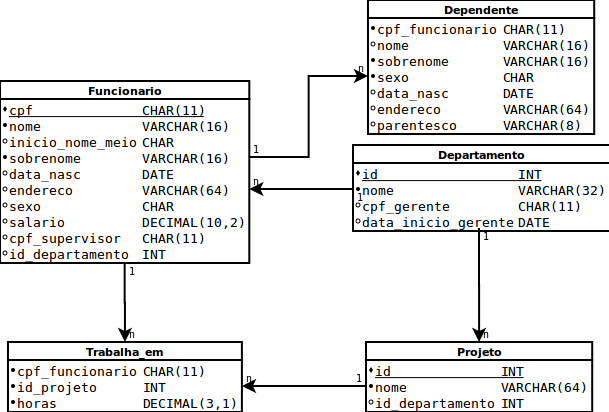
\includegraphics[scale=.4]{../empresa.png}
  \caption{Esquema para o banco de dados {\tt EMPRESA}.}
  \label{fig:empresa}
\end{figure}

\exercise~(Elmasri \& Navathe.) Para o modelo de dados empresa descrito na
Figura~\ref{fig:empresa}, especifique as seguintes consultas:

\begin{enumerate}[a)]
\item Recupere os nomes de todos os funcionários que trabalham no
  departamento que tem o funcionário com o maior salário entre todos
  os funcionários.
\item Recupere o nome de todos os funcionários que ganhem pelo menos
  10.000,00 a mais que o funcionário que recebe menos na empresa.
\end{enumerate}

\exercise~A partir da tabela @code{Aluno} descrita a seguir, crie um gatilho
que remova a entrada de um aluno da tabela quando ele se forma. Leve em consideração 
que o curso tem duração de 8 semestres.

\begin{verbatim}
CREATE TABLE Aluno (
  id INT PRIMARY KEY NOT NULL,
  nome VARCHAR(64) NOT NULL,
  curso VARCHAR(32) NOT NULL,
  semestre INT NOT NULL
);
\end{verbatim}

% Fonte: http://pgbr.postgresql.org.br/2009/palestras/aud1/plpgsql-roberto-mello.pdf
\exercise~(Roberto Mello.) Crie as tabelas a seguir:

\begin{verbatim}
CREATE TABLE vendedor(
    id SERIAL NOT NULL PRIMARY KEY, 
    nome VARCHAR(256)
);
CREATE TABLE venda(
    item_id INTEGER, 
    vendedor_id INTEGER REFERENCES vendedor(id), 
    quantidade INTEGER NOT NULL, 
    valor NUMERIC NOT NULL -- valor total não unitário
);
\end{verbatim}
 
 Escreva um gatilho ({\em trigger}) que insira um novo 
registro na tabela {\tt comissao} de 20\% do valor da venda, quando um
vendedor fizer uma {\tt venda} cujo valor seja maior que
R\$~450,00. Utilize o seguinte modelo de dados para a tabela {\tt
comissao}:
\begin{verbatim}
CREATE TABLE comissao(
    id SERIAL NOT NULL PRIMARY KEY, 
    vendedor_id INTEGER REFERENCES vendedor(id), 
    item_id INTEGER NOT NULL, 
    valor NUMERIC NOT NULL
);
\end{verbatim}

\exercise~Escreva funções ({\em stored procedures}) que realizem as seguintes
ações:

\begin{enumerate}[a)]
\item Receba um valor inteiro e decrementa somente se o valor for maior que 0.
\item Receba um número varável de parâmetros e calcule a média, desvio padrão e
  variância.
\end{enumerate}

\exercise~Dê exemplo e descreva o comportamento do comando {\tt LOCK TABLE}.
Qual a diferença para o comando {\tt SELECT FOR UPDATE}?

\exercise~O que acontece se executarmos o comando a seguir na tabela {\tt Funcionario}?

\begin{verbatim}
CREATE INDEX i_funcionario_cpf ON Funcionario(cpf);
\end{verbatim}

\exercise~Qual a diferença entre {\tt OUTER JOIN}, {\tt LEFT JOIN} e {\tt RIGHT JOIN}?


